\section{Random-Access Memory}
\label{sec:ram}

\textit{A memory unit is a collection of storage cells}, together with associated circuits needed to transfer information into and out of a device. The architecture of memory is such that information can be selectively retrieved from any of its internal locations. The time it takes to transfer information to or from any desired random location is always the same -hence the name random-access memory, abbreviated RAM. In contrast, the time required to retrieve information that is stored on magnetic tape depends on the location of the data.

A memory unit stores binary information in groups of bits called \textbf{\textit{words}}. A \textit{word in memory is a set of bits that move in and out of storage as a unit}. A memory word is a group of 1's and 0's and may represent a number, an instruction, one or more alphanumeric characters, or any other binary-coded information. \textit{A group of 8 bits is called a byte}. Most computer memories use words that are multiples of 8 bits in length. The capacity of a memory unit is usually stated as the total number of bytes that the unit can store.

Communication between memory and its environment is achieved through \textit{data input} and \textit{output lines}, \textit{address selection lines}, and \textit{control lines} that specify the direction of transfer. A block diagram of a memory unit is shown in Fig. 2. 
\begin{figure}[H]
  \centering
  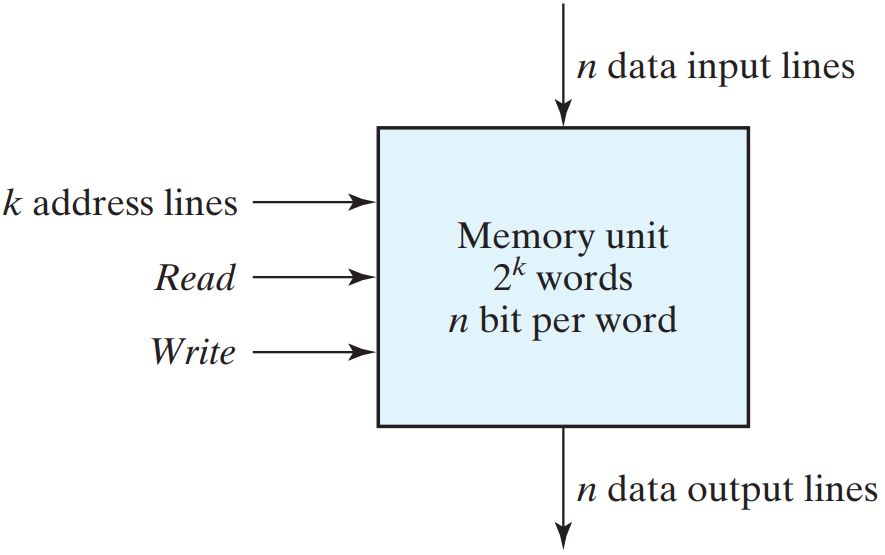
\includegraphics[width=\linewidth]{img/fig-7.2.png}
  \caption{Block diagram of a memory unit}
  \label{fig:7.2}
\end{figure}
\noindent The $n$ data input lines provide the information to be stored in memory, and the $n$ data output lines supply the information coming out of memory. The $k$ address lines specify the particular word chosen among the many available. The two control inputs specify the direction of transfer 
desired: The \textit{Write} input causes binary data to be transferred into the memory, and the \textit{Read} input causes binary data to be transferred out of memory.

The \textit{memory unit is specified by the number of words it contains and the number of bits in each word} ($cell\_size \times word\_size$). The address lines select one particular word. Each word in memory is assigned an identification number, called an address, starting from 0 up to $2^{k - 1}$, where $k$ is the number of address lines.v

The $1K \times 16$ memory of Fig. 3 has 10 bits in the address and 16 bits in each word. Figure 3 shows possible contents of the first three and the last three words of this memory. Each word contains 16 bits that can be divided into two bytes.
\begin{figure}[H]
  \centering
  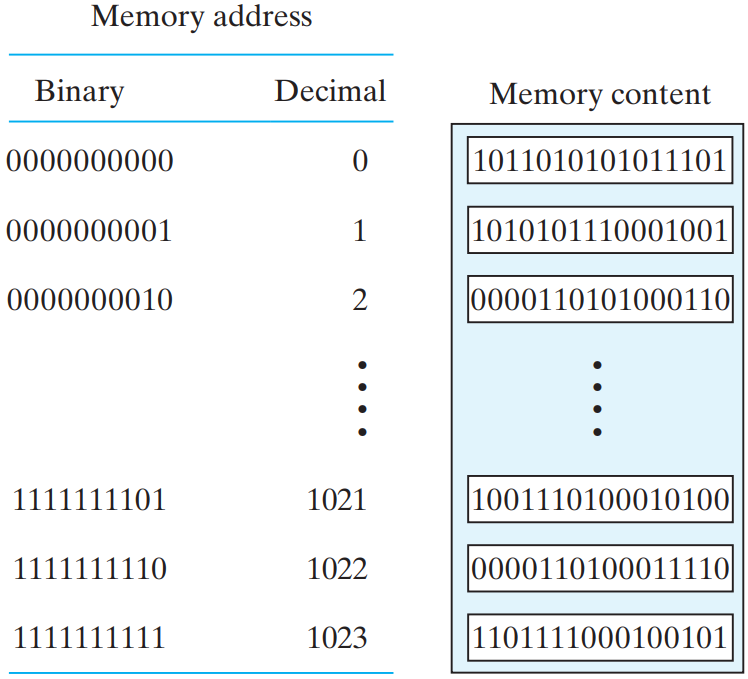
\includegraphics[width=\linewidth]{img/fig-7.3.png}
  \caption{Contents of a $1024 \times 16$ memory}
  \label{fig:7.3}
\end{figure}
\textit{The number of address bits needed in a memory is dependent on the total number of words that can be stored in the memory and is independent of the number of bits in each word}. The number of bits in the address is determined from the relationship $2^k \geq m$, where $m$ is the total number of words and $k$ is the number of address bits needed to satisfy the relationship.


\subsection{Write and Read Operations}
\label{subsec:write-read-operations}

The two operations that RAM can perform are the write and read operations. The write signal specifies a transfer-in operation and the read signal specifies a transfer-out operation. On accepting one of these control signals, the internal circuits inside the memory provide the desired operation.

The steps that must be taken for the purpose of transferring a new word to be stored into memory are as follows:
\begin{enumerate}
  \item Apply the binary address of the desired word to the address lines.
  \item Apply the data bits that must be stored in memory to the data input lines.
  \item Activate the \textit{write} input.
\end{enumerate}
\noindent The memory unit will then take the bits from the input data lines and store them in the word specified by the address lines.

The steps that must be taken for the purpose of transferring a stored word out of memory are as follows:
\begin{enumerate}
  \item Apply the binary address of the desired word to the address lines.
  \item Activate the read input.
\end{enumerate}
The memory unit will then take the bits from the word that has been selected by the address and apply them to the output data lines. The contents of the selected word do not change after the read operation, that is, the read operation is nondestructive.

Most integrated circuits provide two other control inputs: One input selects the unit and the other determines the operation. The memory operations that result from these control inputs are specified in Table 7.1.
\begin{figure}[H]
  \centering
  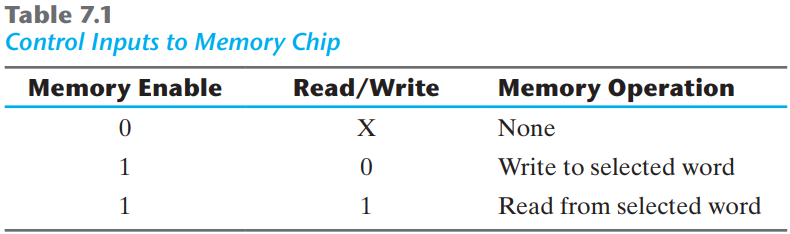
\includegraphics[width=\linewidth]{img/table-7.1.png}
  \label{table:7.1}
\end{figure}


\subsection{Timing Waveforms}
\label{subsec:timing-waveforms}

The operation of the memory unit is controlled by an external device such as a central processing unit (CPU). The CPU is usually synchronized by its own clock. The memory, however, does not employ an internal clock. Instead, its read and write operations are specified by control inputs.

The \textbf{\textit{access time}} of memory is the \textit{time required to select a word and read it}. The \textit{\textbf{cycle time}} of memory is the \textit{time required to complete a write operation}.

The CPU must provide the memory control signals in such a way as to synchronize its internal clocked operations with the read and write operations of memory. This means that the access time and cycle time of the memory must be within a time equal to a fixed number of CPU clock cycles.

The memory timing shown in Fig. 4 is for a CPU with a 50 MHz clock and a memory with 50 ns maximum cycle time. The write cycle in part (a) shows three 20 ns cycles: $T_1$, $T_2$, and $T_3$. For a write operation, the CPU must provide the address and input data to the memory. This is done at the beginning of $T_1$.

The memory enable and the read/write signals must be activated after the signals in the address lines are stable in order to avoid destroying data in other memory words. The memory enable signal switches to the high level and the read/write signal switches to the low level to indicate a write operation.

The two control signals must stay active for at least 50 ns. The address and data signals must remain stable for a short time after the control signals are deactivated. At the completion of the third clock cycle, the memory write operation is completed and the CPU can access the memory again with the next $T_1$ cycle.

The read cycle shown in Fig. 4(b) has an address for the memory provided by the CPU. The memory enable and read/write signals must be in their high level for a read operation. The memory places the data of the word selected by the address into the output data lines within a 50 ns interval (or less) from the time that the memory enable is activated. The CPU can transfer the data into one of its internal registers during the negative transition of $T_3$. The next $T_1$ cycle is available for another memory request.
\vspace*{\fill}
\columnbreak
\begin{figure}[H]
  \centering
  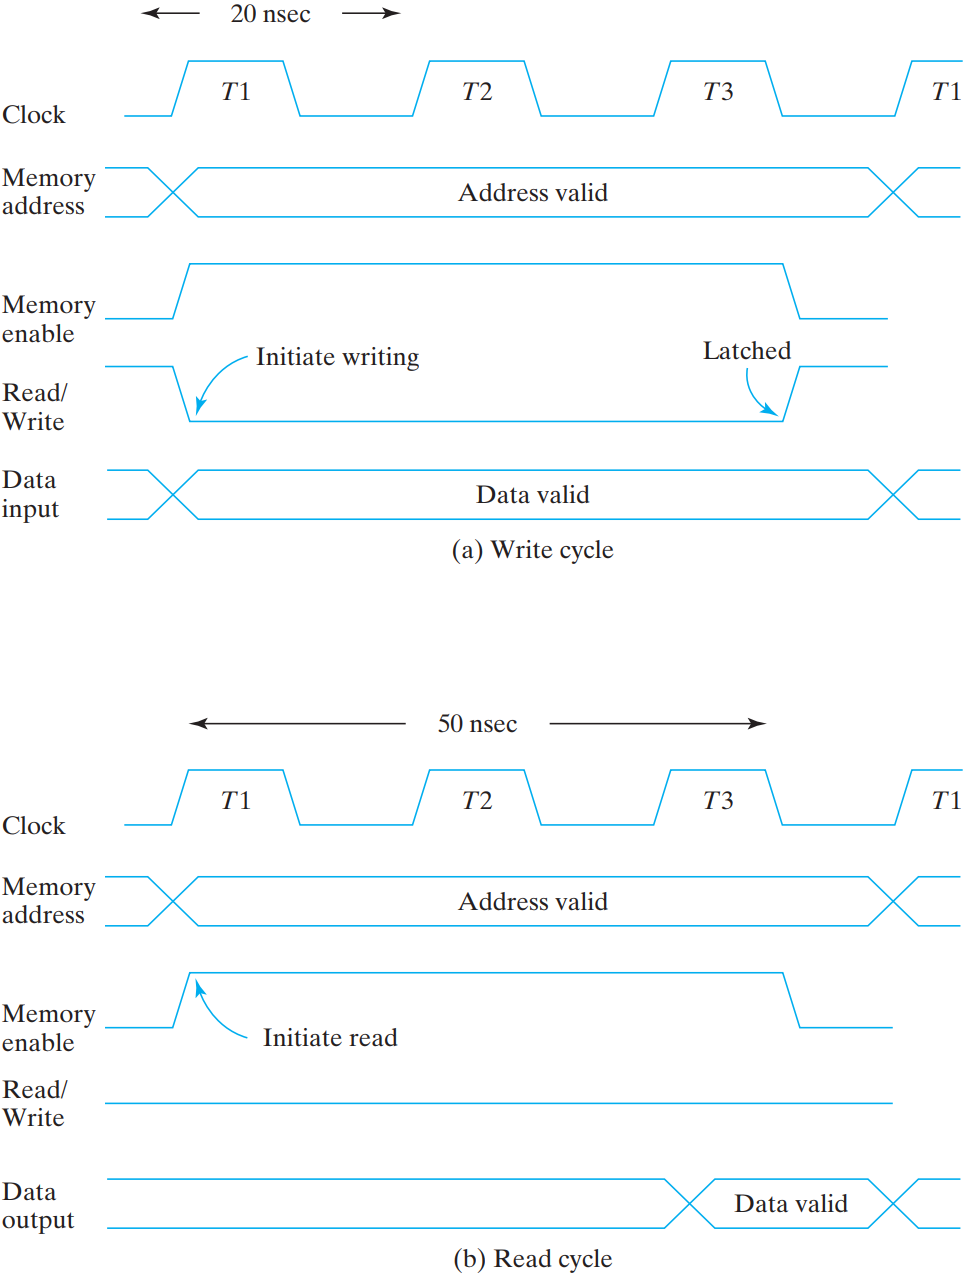
\includegraphics[width=\linewidth]{img/fig-7.4.png}
  \caption{Memory cycle timing waveforms}
  \label{fig:7.4}
\end{figure}


\subsection{Types of Memories}
\label{subsec:types-of-memories}

Integrated circuit RAM units are available in two operating modes: \textit{static} and \textit{dynamic}. 
\begin{itemize}
  \item \textit{\textbf{Static RAM}} (\textit{SRAM}) consists essentially of \textit{internal latches that store the binary information}. The stored information remains valid as long as power is applied to the unit.
  \item \textit{\textbf{Dynamic RAM}} (\textit{DRAM}) \textit{stores the binary information in the form of electric charges on capacitors} provided inside the chip by MOS transistors. The stored charge on the capacitors tends to discharge with time, and the capacitors must be periodically recharged by \textit{refreshing} the dynamic memory.
\end{itemize} 

Refreshing is done by cycling through the words every few milliseconds to restore the decaying charge. DRAM offers reduced power consumption and larger storage capacity in a single memory chip. SRAM is easier to use and has shorter read and write cycles.

The reason why latches are used in SRAM is that a latch can be made with only two NAND or two NOR gates, but a flip-flop requires at least twice that much hardware. Also, in general, smaller is faster, cheaper and requires less power.

Dynamic RAMs tend to be physically smaller than static RAMs. So, this means dynamic RAM is cheaper and denser—more bits can be stored in the same physical area. DRAM offers reduced power consumption and larger storage capacity in a single memory chip.
